\section[Model Universes]{\hyperlink{toc}{Model Universes}}
\subsection{Redshift in single-component universes}
We can take Eq. 5.47 in Ryden as our starting point:
\begin{equation}\label{start51}
    1 + z = \frac{a(t_0)}{a(t_e)} = \left(\frac{t_0}{t_e}\right)^{2/(3 + 3w)}
\end{equation}
Taking the derivative w.r.t. $t_0$ of both sides of this equation, we obtain:
\begin{equation}\label{51temp1}
    \dod{z}{t_0} = \frac{\dot{a}(t_0)\dod{t_0}{t_0}a(t_e) - \dot{a}(t_e)\dod{t_e}{t_0}a(t_0)}{a(t_e)^2}
\end{equation}
There's a variety of terms to process here. First, combining Ryden Eqs. 5.39 and 5.42 we get:
\begin{equation}
    a(t) = \left(\frac{t}{t_O}\right)^{2/(3+3w)}
\end{equation}
Where $t_O$ is the age of the universe. Taking the time derivative, we have:
\begin{equation}\label{dota51}
    \dot{a}(t) = \frac{2}{3+3w}\left(\frac{t}{t_O}\right)^{2/(3+3w)}\frac{1}{t} = \frac{2}{3+3w}\frac{a(t)}{t}
\end{equation}
We also have that:
\begin{equation}\label{t051}
    \dod{t_0}{t_0} = 1
\end{equation}
The final quantity to determine is $\od{t_e}{t_0}$. To solve for this, we recall Ryden 3.59:
\begin{equation}
    \frac{1}{a(t_e)}\int_{t_e}^{t_e + \lambda_e/c}dt = \frac{1}{a(t_0)}\int_{t_0}^{t_0 + \lambda_0/c}
\end{equation}
Since $\lambda/c \ll 1$, we can approximate $\lambda_e/c \sim dt_e$, $\lambda_0/c \sim dt_0$ to get:
\begin{equation}
    \frac{1}{a(t_e)}\int_{t_e}^{t_e + dt_e} dt = \frac{1}{a(t_0)}\int_{t_0}^{t_0 + dt_0}dt
\end{equation}
Which solving the integrals tells us that:
\begin{equation}
    \frac{dt_e}{a(t_e)} = \frac{dt_0}{a(t_0)}
\end{equation}
Which we can rearrange to obtain:
\begin{equation}\label{te51}
    \dod{t_e}{t_0} = \frac{a(t_e)}{a(t_0)} = \frac{1}{1+z}
\end{equation}
Combining the three obtained relations of \eqref{dota51}, \eqref{t051}, \eqref{te51} and substituting this into \eqref{51temp1} we have that:
\begin{equation}
    \dod{z}{t_0} = \frac{\frac{2}{3+3w}\frac{a(t_0)}{t_0}a(t_e) - \frac{2}{3+3w}\frac{a(t_e)}{t_e}\frac{1}{1+z}a(t_0)}{a(t_e)^2}
\end{equation}
Factoring and using that $\frac{a(t_0)}{a(t_e)} = 1 + z$ from \eqref{start51} this becomes:
\begin{equation}
    \dod{z}{t_0} = \frac{2}{3+3w}\left((1+z)\frac{1}{t_0} - \frac{1}{t_e}\right)
\end{equation}
Substituting $t_e = t_0 (1+z)^{-(3+3w)/2}$ from \eqref{start51} we have:
\begin{equation}
    \dod{z}{t_0} = \frac{2}{3+3w}\left((1+z)\frac{1}{t_0} - (1+z)^{(3+3w)/2}\frac{1}{t_0}\right)
\end{equation}
Now using Ryden Eq. 5.42:
\begin{equation}
    t_0 = \frac{2}{3 + 3w}H_0^{-1}
\end{equation}
We obtain:
\begin{equation}
    \boxed{\dod{z}{t_0} = H_0(1+z) - H_0(1+z)^{(3+3w)/2}}
\end{equation}
which was the desired relation. The observed redshift increases in time if $\od{z}{t_0} > 0$, so rearranging the above expression we have:
\begin{equation}
    H_0(1+z) - H_0(1+z)^{(3+3w)/2} > 0 \implies (1+z) > (1+z)^{(3+3w)/2}
\end{equation}
And since $1 + z \geq 1$, the LHS is greater than the RHS if $(3 + 3w)/2 < 1$, i.e. if:
\begin{equation}
    \boxed{w < -\frac{1}{3}}.
\end{equation}

\subsection{Redshift Change Timescale for Flat Matter-Only Universe}
In a flat matter-only universe, we can use the result from 5.1 with $w = 0$ to obtain that:
\begin{equation}
    \dod{z}{t_0} = H_0(1 + z) - H_0(1 + z)^{3/2}
\end{equation}
We want to find the time $dt_0$ for the galaxy to change by $\frac{dz}{z} = -10^{-6}$, and since $z = 1$ to start $dz = -10^{-6}$. Rearranging the above expression to solve for $dt_0$ we have:
\begin{equation}
    dt_0 = \frac{dz}{H_0}\frac{1}{(1+z)-(1+z)^{3/2}}
\end{equation}
So plugging in $dz = -10^{-6}$, $z = 1$, and $H_0 = 68 \si{km s^{-1}Mpc^{-1}}$ we numerically get:
\begin{equation}
    \boxed{dt_0 \approx 5.49 \times 10^{11}\si{s} \approx 17400\si{yrs}}
\end{equation}
\subsection{Present age of universe for positively curved matter-only universe}
We recall the parametric solutions for the scale factor $a$ and the time $t$ for a positively curved universe filled only with matter:
\begin{equation}\label{scale53}
    a(\theta) = \frac{1}{2}\frac{\Omega_0}{\Omega_0 - 1}(1 - \cos\theta)
\end{equation}
\begin{equation}\label{t53}
    t(\theta) = \frac{1}{2H_0}\frac{\Omega_0}{(\Omega_0 - 1)^{3/2}}(\theta - \sin\theta).
\end{equation}
In the present day, $a = 1$, so solving \eqref{scale53} for $\theta$ we have:
\begin{equation}
   \theta = \cos^{-1}\left(1 - \frac{2(\Omega_0 - 1)}{\Omega_0}\right) = \cos^{-1}\left(\frac{2 - \Omega_0}{\Omega_0}\right)
\end{equation}
Substituting this into \eqref{t53} we have:
\begin{equation}\label{t053temp}
    t_0 = \frac{1}{2H_0}\frac{\Omega_0}{(\Omega_0 - 1)^{3/2}}(\cos^{-1}\left(\frac{2 - \Omega_0}{\Omega_0}\right) - \sin(\cos^{-1}\left(\frac{2 - \Omega_0}{\Omega_0}\right)))
\end{equation}
The last term looks complicated, but we can view $\cos^{-1}\left(\frac{2 - \Omega_0}{\Omega_0}\right)$ as the angle for a triangle with hypotenuse $\Omega_0$ and adjacent side $2 - \Omega_0$. The sine of this will therefore be the ratio of the opposite side and the hypotenuse of this triangle. The length of the opposite side is given (by Pythagoras) as:
\begin{equation}
    \sqrt{\Omega_0^2 - (2 - \Omega_0)^2} = 2\sqrt{\Omega_0 - 1}
\end{equation}
So $\sin(\cos^{-1}\left(\frac{2 - \Omega_0}{\Omega_0}\right))$ is given as:
\begin{equation}
    \sin(\cos^{-1}\left(\frac{2 - \Omega_0}{\Omega_0}\right)) = \frac{2\sqrt{\Omega_0 - 1}}{\Omega_0}.
\end{equation}
So substituting this into \eqref{t053temp} we get:
\begin{equation}
    H_0t_0 = \frac{1}{2}\frac{\Omega_0}{(\Omega_0 - 1)^{3/2}}(\cos^{-1}\left(\frac{2 - \Omega_0}{\Omega_0}\right) - \frac{2\sqrt{\Omega_0 - 1}}{\Omega_0})
\end{equation}
Which distributing the product we get:
\begin{equation}
    \boxed{H_0t_0 = \frac{1}{2}\frac{\Omega_0}{(\Omega_0 - 1)^{3/2}}\cos^{-1}\left(\frac{2 - \Omega_0}{\Omega_0}\right) - \frac{1}{\Omega_0 - 1}}
\end{equation}
which was the desired expression. A plot of $t_0$ vs. $\Omega_0$ for $1 \leq \Omega_0 \leq 3$ is given below.

\begin{figure}[htbp]
    \centering
    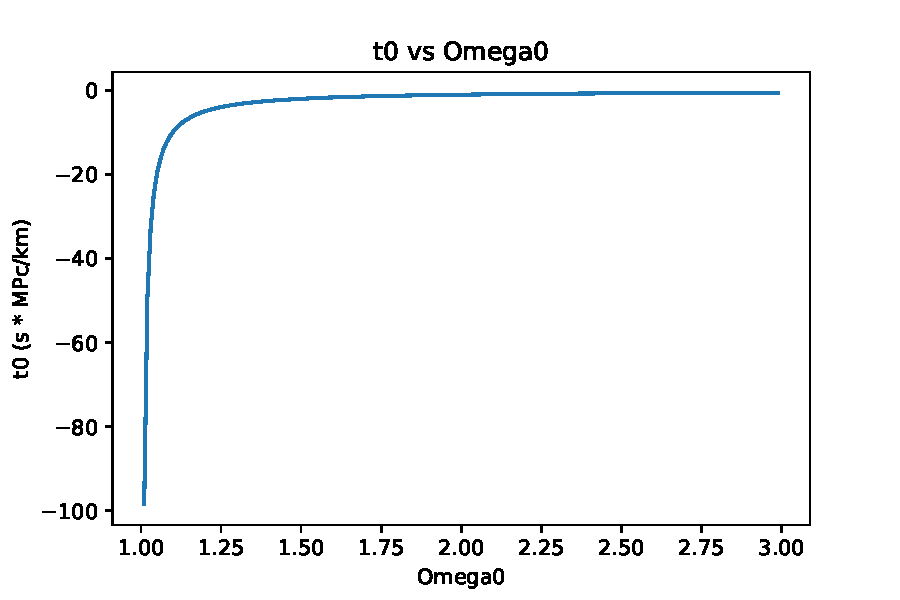
\includegraphics[scale=0.7]{Images/Q5-3.pdf}
    \caption{Plot of $t_0$ vs. $\Omega_0$ for $1 \leq \Omega_0 \leq 3$.}
    \label{plot53}
\end{figure}

\newpage 
\subsection{Present age of universe for negatively curved matter-only universe}
We recall the parametric solutions for the scale factor $a$ and the time $t$ for a negatively curved universe filled only with matter:
\begin{equation}\label{scale54}
    a(\eta) = \frac{1}{2}\frac{\Omega_0}{1 - \Omega_0}(\cosh\eta - 1)
\end{equation}
\begin{equation}\label{t54}
    t(\eta) = \frac{1}{2H_0}\frac{\Omega_0}{(1 - \Omega_0)^{3/2}}(\sinh\eta - \eta).
\end{equation}
In the present day, $a = 1$, so solving \eqref{scale54} for $\eta$ we have:
\begin{equation}
    \eta = \cosh^{-1}\left(\frac{2(1 - \Omega_0)}{\Omega_0} + 1\right) = \cosh^{-1}\left(\frac{2 - \Omega_0}{\Omega_0}\right)
\end{equation}
Substituting this into \eqref{t54} we get:
\begin{equation}
    t_0 = \frac{1}{2H_0}\frac{\Omega_0}{(1 - \Omega_0)^{3/2}}(\sinh( \cosh^{-1}\left(\frac{2 - \Omega_0}{\Omega_0}\right)) - \cosh^{-1}\left(\frac{2 - \Omega_0}{\Omega_0}\right))
\end{equation}
Now, using that $\sinh(\cosh^{-1}x) = \sqrt{x^2 - 1}$, the first term of the above expression becomes:
\begin{equation}
    \sinh( \cosh^{-1}\left(\frac{2 - \Omega_0}{\Omega_0}\right)) = \left(\frac{(2 - \Omega_0)^2}{\Omega_0^2} - 1\right)^{1/2} = \left(\frac{4 - 4\Omega_0}{\Omega_0^2}\right)^{1/2} = \frac{2}{\Omega_0}(1 - \Omega_0)^{1/2}
\end{equation}
So substituting this result we obtain:
\begin{equation}
    H_0t_0 = \frac{1}{2}\frac{\Omega_0}{(1 - \Omega_0)^{3/2}}\left(\frac{2}{\Omega_0}(1 - \Omega_0)^{1/2} - \cosh^{-1}\left(\frac{2 - \Omega_0}{\Omega_0}\right)\right)
\end{equation}
Distributing the terms, we obtain the desired result:
\begin{equation}
    \boxed{H_0t_0 = \frac{1}{1 - \Omega_0} - \frac{\Omega_0}{2(1 - \Omega_0)^{3/2}}\cosh^{-1}\left(\frac{2 - \Omega_0}{\Omega_0}\right)}.
\end{equation}
Finally, a plot of $t_0$ vs. $\Omega_0$ for $0 \leq \Omega_0 \leq 1$ is given below.

\begin{figure}[htbp]
    \centering
    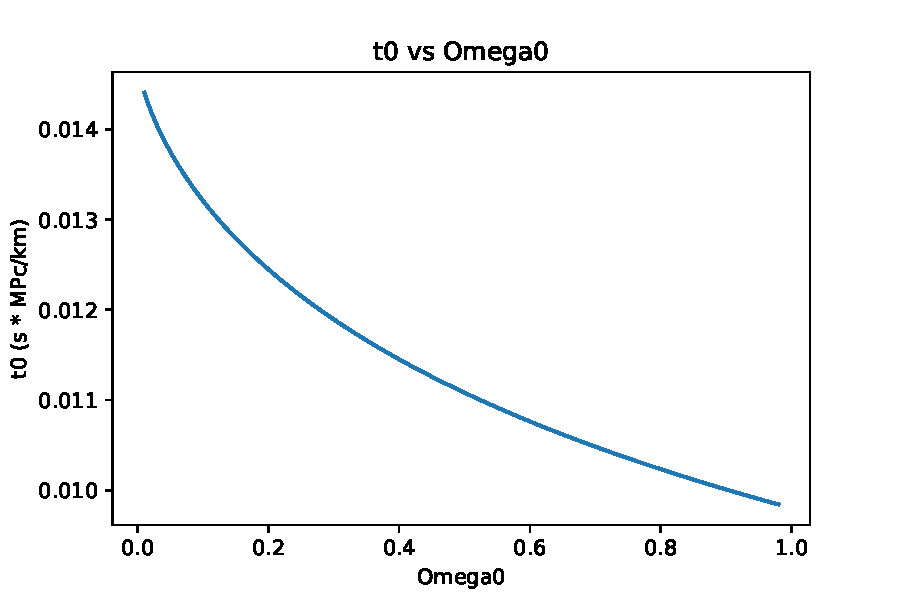
\includegraphics[scale=0.7]{Images/Q5-4.pdf}
    \caption{Plot of $t_0$ vs. $\Omega_0$ for $0 \leq \Omega_0 \leq 1$.}
    \label{plot54}
\end{figure}

\subsection{Phantom Energy and the Big Rip}
The supposed ``phantom energy'' with equation of state parameter $w_p < -1$ would have energy density:
\begin{equation}
    \e_p(a) = \e_{p, 0}a^{-3(1+w_p)}.
\end{equation}
Comparitively, matter has energy density:
\begin{equation}
    \e_{m}(a) = \e_{m, 0}a^{-3}.
\end{equation}
At equality, we have that:
\begin{equation}
    1 = \frac{\e_{p}(a)}{\e_{m}(a)} = \frac{\e_{p, 0}a^{-3(1+w_p)}}{\e_{m, 0}a^{-3}} = \frac{\Omega_{p, 0}}{\Omega_{m, 0}}\frac{1}{a^{3w_p}}
\end{equation}
Since $\Omega_{p, 0} = 1 - \Omega_{m, 0}$, we have:
\begin{equation}
    1 = \frac{1 - \Omega_{m, 0}}{\Omega_{m, 0}}\frac{1}{a^{3w_p}}
\end{equation}
Which we can rearrange to solve for the scale factor $a_{mp}$ where equality holds:
\begin{equation}
    \boxed{a_{mp} = \left(\frac{1}{\Omega_{m, 0}} - 1\right)^{1/3w_p}}
\end{equation}
The Friedmann equation in this universe reads:
\begin{equation}
    \frac{H^2}{H_0^2} = \frac{\Omega_{m, 0}}{a^3} + \frac{\Omega_{p, 0}}{a^{3(1+w_p)}} = \frac{\Omega_{m, 0}}{a^3} + \frac{1 - \Omega_{m, 0}}{a^{3(1+w_p)}}
\end{equation}
In the limit $a \gg a_{mp}$, the first term becomes negligeble and hence:
\begin{equation}
    \frac{H^2}{H_0^2} \approx \frac{1 - \Omega_{m, 0}}{a^{3(1+w_p)}}
\end{equation}
We now rearrange this equation to set up for the integration:
\begin{equation}
    \frac{\frac{\dot{a}}{a}}{H_0} \approx \frac{(1 - \Omega_{m, 0})^{1/2}}{a^{3(1+w_p)/2}} \implies H_0 dt \approx a^{3(1+w_p)/2}(1 - \Omega_{m, 0})^{-1/2}da
\end{equation}
Integrating from $t_0$ to $t_{rip}$, corresponding to from $ a(t_0) = 1$ to $a(t_{\text{rip}}) = \infty$ on the RHS, we have:
\begin{equation}
    \int_{t_0}^{t_{\text{rip}}}H_0 dt  \approx \int_1^\infty a^{3(1+w_p)/2}(1 - \Omega_{m, 0})^{-1/2}da
\end{equation}
Carrying out the integral, we get:
\begin{equation}
    H_0(t_{\text{rip}} - t_0) \approx \left. \frac{2}{3(1+w_p)}a^{3(1+w_p)/2}(1 - \Omega_{m, 0})^{-1/2}\right|_{1}^\infty
\end{equation}
Since $w_p < -1$, the RHS goes to $0$ at $a = \infty$, so:
\begin{equation}
    H_0(t_{\text{rip}} - t_0) \approx -\frac{2}{3(1+w_p)}(1 - \Omega_{m, 0})^{-1/2}
\end{equation}
Which we can write as:
\begin{equation}
    \boxed{H_0(t_{\text{rip}} - t_0) \approx \frac{2}{3\abs{1+w_p}}(1 - \Omega_{m, 0})^{-1/2}}
\end{equation}
which was the desired result. Finally, with $H_0 = 68\si{km.s^{-1}.Mpc^{-1}}, \Omega_{m, 0} = 0.3$, and $w_p = -1.1$, we can solve numerically for the time remaining until the ``Big Rip'' to be:
\begin{equation}
    \boxed{t_{\text{rip}} - t_0 \approx 2.53 \times 10^{18}\si{s} = 80.4 \times 10^{10}\si{yrs}}
\end{equation}

\subsection{Pulling an Einstein}
In this universe with matter and dark energy, the acceleration equation reads:
\begin{equation}
    \frac{\ddot{a}}{a} = -\frac{4\pi G}{3c^2}(\e + 3P) = -\frac{4\pi G}{3c^2}(\e_m + \e_q + 3w_q \e_q)
\end{equation}
Where we have used that $P = (0)\e_m = 0$ for matter and $P = w_q\e_q$ for the dark energy. To have a static universe with $\ddot{a} = 0$, it must follow that:
\begin{equation}
    \boxed{\e_m = -(1 + 3w_q)\e_q}
\end{equation}
The Friedmann equation reads:
\begin{equation}
    H(t)^2 = \frac{8\pi G}{3c^2}(\e_m + \e_q) - \frac{\kappa c^2}{R_0^2a(t)^2}
\end{equation}
Since we have a static universe, $\dot{a} = 0$ and hence $H(t) = 0$. Furthermore, using that $\e_m = -(1 + 3w_q)\e_q$ from earlier, the Friedmann equation becomes:
\begin{equation}
    0 = \frac{8\pi G}{3c^2}(-3w_q)\e_q - \frac{\kappa c^2}{R_0^2a(t)^2}
\end{equation}
Since $-1 < w_q < -1/3$, $w_q$ is negative, and hence the only way the above equality is satisfied is if $\kappa = 1$ so the positive term can be cancelled by the second term. So in this scenario, $\boxed{\text{the universe is positively curved}}$. We rearrange the above equation to solve for the radius of curvature $R_0$ when $a(t) = 1$:
\begin{equation}
    \boxed{R_0 = \sqrt{\frac{c^4}{8\pi G \abs{w_q} \e_q}}}
\end{equation}

\subsection{Big Crunch}
For a positively curved matter only universe, we recall the parametric solutions for $a(\theta), t(\theta)$ (Ryden Eqs. 5.90/5.91):
\begin{equation}
    a(\theta) = \frac{1}{2}\frac{\Omega_0}{\Omega_0 - 1}(1 - \cos\theta)
\end{equation}
\begin{equation}
    t(\theta) = \frac{1}{2H_0}\frac{\Omega_0}{(\Omega_0 - 1)^{3/2}}(\theta - \sin\theta)
\end{equation}
The big bang occurs at $\theta = 0$, and the Big crunch at $\theta = 2\pi$. Given the parametric solutions above, he time between these can be computed as (Ryden Eq. 5.92):
\begin{equation}
    t_{\text{crunch}} = \frac{\pi}{H_0}\frac{\Omega_0}{(\Omega_0 - 1)^{3/2}}
\end{equation}
Furthermore, we can solve for the present $t_0$ at which $a(\theta_0) = 1$:
\begin{equation}\label{theta0}
    a(\theta_0) = 1 = \frac{1}{2}\frac{\Omega_0}{\Omega_0 - 1}(1 - \cos\theta_0) \implies \theta_0 = \arccos\left(1 - \frac{2(\Omega_0 - 1)}{\Omega_0}\right) = \arccos\left(\frac{2}{\Omega_0} - 1\right)
\end{equation}
Therefore the time between Dr. Niwde's obsdrvations at $t = t_0 = t(\theta_0)$ and the final big crunch is given by:
\begin{equation}
    \Delta t = t_{\text{crunch}} - t(\theta_0) = \frac{\pi}{H_0}\frac{\Omega_0}{(\Omega_0 - 1)^{3/2}} - \frac{1}{2H_0}\frac{\Omega_0}{(\Omega_0 - 1)^{3/2}}(\theta_0 - \sin\theta_0)
\end{equation}
Or more concisely:
\begin{equation}
    \boxed{\Delta t = \frac{1}{H_0}\frac{\Omega}{(\Omega_0 - 1)^{3/2}}\left(\pi - \frac{1}{2}(\theta_0 - \sin\theta_0)\right)}
\end{equation}
Where $\theta_0$ is given in \eqref{theta0}. To determine the highest amplitude blueshift, we recall the redshift-scale factor relation $1 + z = \frac{1}{a}$, so:
\begin{equation}
    z = \frac{1}{a} - 1
\end{equation}
If we want to minimize $z$ (i.e. have it be the most negative/highest magnitude blueshift), we want to maximize $a$. We can determine this from the Friedmann equation (a la Ryden Eq. 5.86) but it also can easily be read off from the parametric solution above to be:
\begin{equation}
    a_{\text{max}} = \frac{\Omega_0}{\Omega_0 - 1}
\end{equation}
which is attained at $\theta = \pi$. So, the highest amplitude blueshift that Dr. Niwde can observe is at:
\begin{equation}
    \boxed{z_{\text{blue, max}} = \frac{\Omega_0 - 1}{\Omega} - 1 = -\frac{1}{\Omega_0}}
\end{equation}
At this blueshift, as stated previously we have $\theta = \pi$. So this occurs at:
\begin{equation}
    t_{\text{blue, max}} = t(\pi) =  \frac{1}{2H_0}\frac{\Omega_0}{(\Omega_0 - 1)^{3/2}}(\pi - \sin\pi) = \frac{\pi}{2H_0}\frac{\Omega_0}{(\Omega_0 - 1)^{3/2}}
\end{equation}
So the lookback time is:
\begin{equation}
   t_0 -  t_{\text{blue, max}} =  \frac{1}{2H_0}\frac{\Omega_0}{(\Omega_0 - 1)^{3/2}}(\theta_0 - \sin\theta_0) - \frac{\pi}{2H_0}\frac{\Omega_0}{(\Omega_0 - 1)^{3/2}}
\end{equation}
Or with some factoring:
\begin{equation}
    \boxed{t_0 -  t_{\text{blue, max}} = \frac{1}{2H_0}\frac{\Omega_0}{(\Omega_0 - 1)^{3/2}} \left(\theta_0 - \sin\theta_0  - 1\right)}
\end{equation}

\subsection{Big Bounce}
The Friedmann equation in such a universe would read:
\begin{equation}\label{Freid58}
    \frac{H^2}{H_0^2} = \Omega_0 + \frac{1 - \Omega_0}{a^2}
\end{equation}
At the point where $a$ has an extrema, $H(t) = 0$ and so:
\begin{equation}
    0 = \Omega_0 + \frac{1 - \Omega_0}{a^2} \implies \boxed{a_{\text{bounce}} = \left(\frac{\Omega_0 - 1}{\Omega_0}\right)^{1/2}}
\end{equation}
Rearranging the Friedmann equation, we have:
\begin{equation}
    \frac{\dot{a}}{a} = H_0\sqrt{\Omega_0}\sqrt{1 - \frac{a_{\text{bounce}}^2}{a^2}} \implies \dod{a}{t} = \frac{H_0}{\sqrt{\Omega_0}}\sqrt{a^2 - a^2_{\text{bounce}}}
\end{equation}
Integrating, we obtain:
\begin{equation}
   \sqrt{\Omega_0} H_0\int_{t_{\text{bounce}}}^{t_0} dt = \int_{a_{\text{bounce}}}^a \frac{1}{\sqrt{a'^2 - a^2_{\text{bounce}}}} da'
\end{equation}
Integrating both sides (making use of an integral table for the RHS), we have:
\begin{equation}\label{58temp}
    \sqrt{\Omega_0} H_0(t - t_{\text{bounce}}) = \arccosh\left(\frac{a}{a_{\text{bounce}}}\right)
\end{equation}
Which we can rearrange to obtain:
\begin{equation}
    \boxed{a(t) = a_{\text{bounce}}\cosh\left(\sqrt{\Omega_0} H_0(t - t_{\text{bounce}})\right)}
\end{equation}
At $t_0$ we have that $a(t_0) = 1$ by convention, so solving for $t_0 - t_{\text{bounce}}$ using \eqref{58temp} we have:
\begin{equation}
    \boxed{t_0 - t_{\text{bounce}} = \frac{1}{H_0\sqrt{\Omega_0}}\arccosh\left(\left(\frac{\Omega_0}{\Omega_0 - 1}\right)^{1/2}\right)}
\end{equation}

\subsection{$\Omega_{m, 0}$ for $t = H_0^{-1}$}
In a spatially flat and matter + cosmological constant filled universe, te Friedmann equation can be integrated to yield the analytic solution relating $t$ and $a$ (Ryden Eq. 5.101):
\begin{equation}\label{analyticmlambda}
    H_0t = \frac{2}{3\sqrt{1 - \Omega_{m, 0}}}\ln\left[\left(\frac{a}{a_{m\Lambda}}\right)^{3/2} + \sqrt{1 + \left(\frac{a}{a_{m\Lambda}}\right)^3}\right]
\end{equation}
Where $a_{m\Lambda}$ is defined by:
\begin{equation}\label{amlambda}
    a_{m\Lambda} = \left(\frac{\Omega_{m,0}}{1 - \Omega_{m, 0}}\right)^{1/3}
\end{equation}
At the present time, we have $t = t_0$, and $a = a(t_0) = 1$ by convention. Substituting this, as well as \eqref{amlambda} into \eqref{analyticmlambda} we get:
\begin{equation}
    H_0t_0 = \frac{2}{3\sqrt{1 - \Omega_{m, 0}}}\ln\left[\sqrt{\frac{1-\Omega_{m, 0}}{\Omega_{m, 0}}} + \sqrt{1 + \frac{1-\Omega_{m, 0}}{\Omega_{m, 0}}}\right]
\end{equation}
In order to have $t_0 = H_0^{-1}$ we require the RHS of the above equation to exactly equal one:
\begin{equation}
    1 = \frac{2}{3\sqrt{1 - \Omega_{m, 0}}}\ln\left[\sqrt{\frac{1-\Omega_{m, 0}}{\Omega_{m, 0}}} + \sqrt{1 + \frac{1-\Omega_{m, 0}}{\Omega_{m, 0}}}\right]
\end{equation}
Rewriting the last term:
\begin{equation}
    1 = \frac{2}{3\sqrt{1 - \Omega_{m, 0}}}\ln\left[\sqrt{\frac{1-\Omega_{m, 0}}{\Omega_{m, 0}}} + \sqrt{\frac{1}{\Omega_{m, 0}}}\right] = \frac{2}{3\sqrt{1 - \Omega_{m, 0}}}\ln\left[\frac{1 + \sqrt{1 - \Omega_{m, 0}}}{\sqrt{\Omega_{m, 0}}}\right]
\end{equation}
Using the hyperbolic secant identity of $\arcsech x = \ln(\frac{1 + \sqrt{1 - x^2}}{x})$, we have:
\begin{equation}
    1 = \frac{2}{3\sqrt{1 - \Omega_{m, 0}}}\arcsech(\sqrt{\Omega_{m, 0}})
\end{equation}
Or:
\begin{equation}\label{59exp}
    \frac{3\sqrt{1 - \Omega_{m, 0}}}{2} = \arcsech(\sqrt{\Omega_{m, 0}})
\end{equation}
This equation can now be solved numerically for $\Omega_{m, 0}$ to find:
\begin{equation}
    \boxed{\Omega_{m, 0} \approx 0.263}
\end{equation}

\subsection{Amounts in the Benchmark model}
In the Benchmark model, we have (from Ryden Table 5.2) that:
\begin{equation}
    \Omega_{m, 0} = 0.31, \quad \Omega_{\gamma, 0} = 5.35 \times 10^{-5},\quad  \Omega_{\text{bary}, 0} = 0.048
\end{equation}
We that $\Omega = \frac{\e(t)}{\e_c(t)}$ where $\e_C$ is the critical density, which is currently $\e_{c, 0} 7.8 \times 10^{-10}\si{J.m^{-3}}$ (up to uncertainty). Therefore obtaining the energy density for photons in the benchmark model, we have:
\begin{equation}
    \e_{\gamma, 0} = \e_{c, 0}\Omega_{\gamma, 0} = 4.17 \times 10^{-14} \si{J.m^{-3}}
\end{equation}
It will be more convenient to solve for the mass density for the matter and baryons:
\begin{equation}
    \rho_{m, 0} = \e_{c, 0}\Omega_{\gamma, 0}/c^2 = 2.69 \times 10^{-27}\si{kg.m^{-3}}, \quad \rho_{\text{bary}, 0} = \e_{c, 0}\Omega_{\text{bary}, 0}/c^2 = 4.16 \times 10^{-28} \si{J.m^{-3}} 
\end{equation}
In addition, in the Benchmark model we have a finite horizon distance (Ryden Eq. 5.115):
\begin{equation}
    d_{\text{hor}}(t_0) = 14000\si{Mpc} = 4.33 \times 10^{26}\si{m}.
\end{equation}
Therefore the volume of the universe within the horizon distance is:
\begin{equation}
    V_{\text{hor}}(t_0) = \frac{4}{3}\pi d_{\text{hor}}(t_0)^3 = 3.39 \times 10^{80} \si{m^3}
\end{equation}
Now, solving for the total mass of all matter within our horizon, we have:
\begin{equation}
    \boxed{M_m =  V_{\text{hor}}(t_0)\rho_{m, 0} = 9.12 \times 10^{53}\si{kg}}
\end{equation}
Next, solving for the total amount of energy of photons within the horizon distance, we have:
\begin{equation}
    \boxed{E_{\text{photons}} = V_{\text{hor}}(t_0)\e_{\gamma, 0} = 1.41 \times 10^{67} \si{J}}
\end{equation}
Finally, we solve for the number of baryons in the universe. This will be the total mass of baryons within the universe divided by the mean mass per Baryon. Approximating baryonic matter as 75\% hydrogen and 25\% helium, we have the mean mass is given by:
\begin{equation}
    m_{\text{avg}} = 0.75m_{\text{H}} + 0.25m_{\text{He}} \approx 0.75(m_p) + 0.25(4m_p) = 1.75m_{p} = 2.92 \times 10^{-27}\si{kg}
\end{equation}
So therefore the total number of baryons within the horizon, we have:
\begin{equation}
    \boxed{N_{\text{bary}} =  V_{\text{hor}}(t_0)\rho_{\text{bary}, 0}/m_{\text{avg}} = 4.83 \times 10^{79} \text{baryons}}
\end{equation}

\subsection*{Time and Scale Factor for Matter-Only Universe}
\addcontentsline{toc}{subsection}{\protect\numberline{}Time and Scale Factor for Matter-Only Universe}
\begin{tcolorbox}
Let's make sure we can work through the mathematical steps for a closed matter-only (i.e. `Matter + Curvature') universe. Try to do this without looking up the book for every step! Start by writing the Friedmann equation for this case, using $a$ rather than $1+z$, and with the single parameter $\Omega_0$ (where this implicitly means `matter', here). Thus write an integral expression for $t$. It may not look trivial to solve this for $t(a)$ or $a(t)$, but you should be able to \emph{show} that the following parametric solution works [a `parametric solution' means that you can write doesn $y(\phi)$ and $x(\phi)$, both in terms of a parameter $\phi$, even if an explicit expression for $y(x)$ is hard or impossible]:
\begin{equation}\label{parametric_a}
    a(\theta) = \frac{1}{2}\frac{\Omega_0}{\Omega_0 - 1}(1-\cos\theta)
\end{equation}
\begin{equation}\label{parametric_t}
    t(\theta) = \frac{1}{2H_0}\frac{\Omega_0}{(\Omega_0 - 1)^{3/2}}(\theta - \sin\theta).
\end{equation}
To be clear: you are being asked to show that in the appropriate Friedmann equation, the LHS is equal to the RHS if you assume the above solution (\emph{or} you could solve the integral, but that's harder!). [You might have to do a bit of rearranging of trig functions - but perservere, because it works!] Lastly, by letting $\theta$ run from $0$ to $2\pi$, sketch $a$ vs. $t$ for this model. 
\end{tcolorbox}

The Friedmann equation in this case reads:
\begin{equation}
    \boxed{\frac{H^2}{H_0^2} = \frac{\Omega_0}{a^3} + \frac{1 - \Omega_0}{a^2}}
\end{equation}
Now, since $H = \frac{\dot{a}}{a}$, we can rearrange this to obtain that:
\begin{equation}\label{friedmann_mat}
    \frac{\dot{a}^2}{H_0^2} = (\frac{\Omega_0}{a} + 1 - \Omega_0)
\end{equation}
Or in other words:
\begin{equation}
    \dod{a}{t} = H_0\sqrt{\frac{\Omega_0}{a} + 1 - \Omega_0}
\end{equation}
So solving for $t$ we integrate:
\begin{equation}
    \boxed{H_0t = \int_0^t dt' = \int_0^a \frac{da'}{\sqrt{\frac{\Omega_0}{a} + 1 - \Omega_0}}}.
\end{equation}
Now, we verify that \eqref{friedmann_mat} holds for the parametric solution given by \eqref{parametric_a} and \eqref{parametric_t}. First, we determine what $\dot{a}$ is given this solution. By the chain rule, we have that:
\begin{equation}
    \dot{a} = \dod{a}{t} = \dod{a}{\theta}\dod{\theta}{t} = \dod{a}{\theta}\dot{\theta}
\end{equation}
Solving for $\od{a}{\theta}$ by differentiating \eqref{parametric_a} we have:
\begin{equation}
    \dod{a}{\theta} = \frac{1}{2}\frac{\Omega_0}{\Omega_0 - 1}\sin\theta.
\end{equation}
And solving for $\dot{theta}$ by implicitly differentiating \eqref{parametric_t} we have:
\begin{equation}
    1 = \frac{1}{2H_0}\frac{\Omega_0}{(\Omega_0 - 1)^{3/2}}(\dot{\theta} - \dot{\theta}\cos\theta) \implies \dot{\theta} = \frac{2H_0(\Omega_0 - 1)^{3/2}}{\Omega_0(1-\cos\theta)}
\end{equation}
Hence, we find that:
\begin{equation}
    \dot{a} = \frac{H_0(\Omega_0 - 1)^{1/2}}{1 - \cos\theta}\sin\theta
\end{equation}
Evaluating the LHS of \eqref{friedmann_mat}, we have:
\begin{equation}\label{LHS_friedmann_mat}
    \frac{\dot{a}^2}{H_0^2} = \frac{\Omega_0 - 1}{(1 - \cos\theta)^2}\sin^2\theta
\end{equation}
Evaluating the RHS of \eqref{friedmann_mat}, we have:
\begin{equation}
    \frac{\Omega_0}{a} + 1 - \Omega_0 = (\frac{\Omega_0}{\frac{1}{2}\frac{\Omega_0}{\Omega_1 - 1}(1-\cos\theta)} + 1 - \Omega_0)
\end{equation}
Multiplying the first term by $1 = \frac{1 - \cos\theta}{1-\cos\theta}$ and the second term by $1 = \left(\frac{1 - \cos\theta}{1-\cos\theta}\right)^2$ we obtain:
\begin{equation}
    \frac{\Omega_0}{a} + 1 - \Omega_0 = \frac{2(\Omega_0 - 1)}{(1 -\cos\theta)^2}(1 - \cos\theta) - \frac{\Omega_0 - 1}{(1 - \cos\theta)^2}(1 - \cos\theta)^2
\end{equation}
Which after some expanding and cancellation, becomes:
\begin{equation}\label{RHS_friedmann_mat}
    \frac{\Omega_0}{a} + 1 - \Omega_0 = \frac{\Omega_0 - 1}{(1 - \cos\theta)^2}(1 -\cos^2\theta)
\end{equation}
Using the famous trig identity $\sin^2\theta + \cos^2\theta = 1$, we can identify \eqref{LHS_friedmann_mat} with \eqref{RHS_friedmann_mat} to conclude that this is indeed the correct solution.

For the plot, we observe that the given parametric equations are exactly of those for a cycloid, so the curve of $t(\theta)$ vs. $a(\theta)$ will be exactly that it is displayed below.

\begin{figure}[htbp]
    \centering
    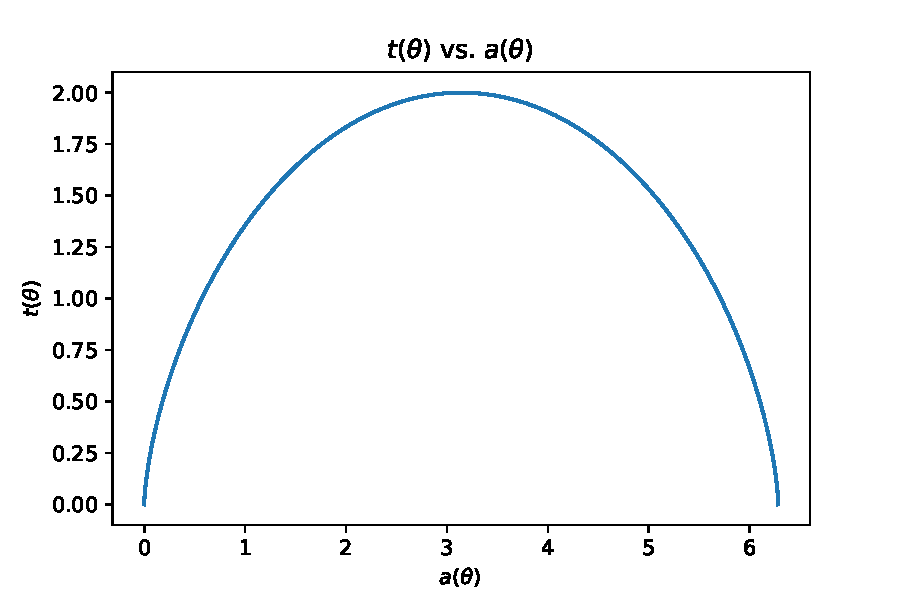
\includegraphics[scale=0.7]{Images/Q5-A.pdf}
    \caption{Plot of $t(\theta)$ vs. $a(\theta)$ for $\theta \in [0, 2\pi)$. $\Omega_0 = 2$ and $H_0 = 1$ were chosen for convenience of plotting.}
    \label{plotatcycloid}
\end{figure}